
\section{Software installation and testing}

Décrire votre travail (environ 6 pages)
\begin{itemize}
	\item architecture de votre solution (vision haut niveau)
	\item implémentation de votre solution (détail technique) ou de la partie la plus intéressante si la place manque

\end{itemize}

In this part I will discuss the diffenrents softwares I have installed for the company. Firstofall I will focus on th research I had to do. Then the details of the installation will be detailed. 
\subsection{Researches}
%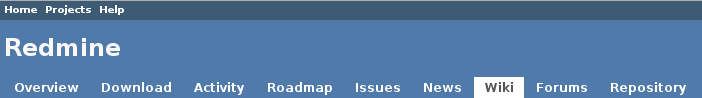
\includegraphics[scale=0.55]{Images/redmine.png} \\

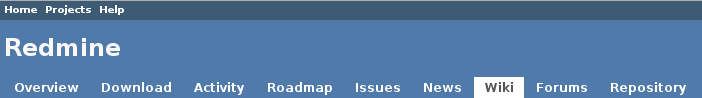
\includegraphics[width=\textwidth]{Images/redmine.png}
\newline
\\
I dind't know a lot about project managing so I had to look what was Redmine for and what this application will allow us to do. 
Redmine is a powerful web based project managing which allow bugs tracking. It is possible to add a lot of functionalities to this application in intalling  some plugings into it. \\ 
I read about all the plugings for Redmine and finally chose some of them  
	\begin{wrapfigure}
		
\includegraphics[scale=0.1]{Images/jenkins.jpeg} 
		Jenkins. \\
		It is an application that monitors executions of repeated jobs such as bulding, testing a software project.
	\end{wrapfigure} 
	\begin{figure}[h]
		
\includegraphics[scale=0.2]{Images/mylin.jpeg} 
		Mylin for eclipse connection
	\end{figure} 
	\begin{figure}[h]
		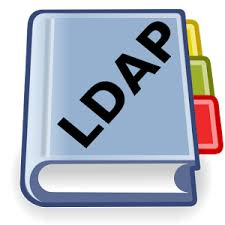
\includegraphics[scale=0.1]{Images/ldap.jpeg} 
		Ldap authentification. \\
		Ldap is a protocol that allow us to access and maintain directory services. So we can access to some informations about the users of a network over TCP/IP protocol. 
		With the ldap authentification into redmine, the users don't need to create an Redmine'es account but they can directly access into their redmine's project by using their ldap password and login.   
	\end{figure} 




\subsection{Implementation}

